%\documentclass[11pt,oneside,a4paper,openright]{report}
%\usepackage[utf8]{inputenc}
%\renewcommand{\contentsname}{Indholdsfortegnelse}
%\usepackage{pdfpages}
%\usepackage{titlesec}
%\titleformat{\chapter}{\normalfont\huge}{\thechapter.}{20pt}{\huge\it}

%%%% Dokumentklassen %%%%

\documentclass[a4paper,11pt,dvipsnames,oneside,openany]{memoir} 	% Openright åbner kapitler på højresider (openany begge)
% fleqn = flush left equation - sikre at alle ligninger tvinges til venstre. I 3. semesterprojektet, skulle ligningerne stå i midten derfor er denne pakke slettet fra dokumentklassen.

\usepackage{subfiles}
\usepackage{nameref}
\usepackage{tabularx}
\usepackage{multirow}
\usepackage[table]{xcolor}


%%%% PACKAGES %%%%

%% Oversættelse og tegnsætning %%
\usepackage[utf8]{inputenc}					% Input-indkodning af tegnsæt (UTF8)
\usepackage[danish]{babel}					% Dokumentets sprog
\usepackage[T1]{fontenc}				    % Output-indkodning af tegnsæt (T1)
\usepackage{ragged2e,anyfontsize}			% Justering af elementer
%\usepackage{fixltx2e}						% Retter forskellige fejl i LaTeX-kernen
\usepackage{titletoc}
\newcommand{\nocontentsline}[3]{}
\newcommand{\tocless}[2]{\bgroup\let\addcontentsline=\nocontentsline#1{#2}\egroup}									% Giver mulighed for at fjerne section nummer i indholdsfortegnelse ved \tocless


\usepackage{lastpage}						% Total antal sider opdateres automatisk ved \pageref{LastPage}
\usepackage{tikz}							% Til at lave flow diagrammer
\usetikzlibrary{calc,trees,positioning,arrows,chains,shapes.geometric,decorations.pathreplacing,decorations.pathmorphing,shapes,matrix,shapes.symbols}				% Til at lave diagrammer
																			
%% Figurer og tabeller (floats) %%
\usepackage{graphicx} 						% Håndtering af eksterne billeder (JPG, PNG, EPS, PDF)
\usepackage{multicol}         	           	% Muliggør output i spalter
\usepackage{rotating}						% Rotation af tekst med \begin{sideways}...\end{sideways}
\usepackage{xcolor}							% Definer farver med \definecolor. Se mere: http://en.wikibooks.org/wiki/LaTeX/Colors
\usepackage{flafter}						% Sørger for at floats ikke optræder i teksten før deres reference
\let\newfloat\relax 						% Justering mellem float-pakken og memoir
\usepackage{float}							% Muliggør eksakt placering af floats, f.eks. \begin{figure}[H]
\usepackage{color, colortbl}				% Tilføjer farve til tabeller

\definecolor{Gray}{gray}{0.9}				% Definerer en farve "yeezy-gray"

%% Matematik mm. %%
\usepackage{amsmath,amssymb,stmaryrd} 		% Avancerede matematik-udvidelser
\usepackage{mathtools}						% Andre matematik- og tegnudvidelser
\usepackage{textcomp}                 		% Symbol-udvidelser (fx promille-tegn med \textperthousand)
\usepackage{rsphrase}						% Kemi-pakke til RS-saetninger, fx \rsphrase{R1}
\usepackage[version=3]{mhchem} 				% Kemi-pakke til flot og let notation af formler, f.eks. \ce{Fe2O3}
\usepackage{siunitx}						% Flot og konsistent præsentation af tal og enheder med \si{enhed} og \SI{tal}{enhed}
\sisetup{output-decimal-marker = {,}}		% Opsætning af \SI (DE for komma som decimalseparator) 

%% Referencer og kilder %%
\usepackage[danish]{varioref}				% Muliggør bl.a. krydshenvisninger med sidetal (\vref)
\usepackage{natbib}							% Udvidelse med naturvidenskabelige citationsmodeller
\usepackage{xr}							    % Referencer til eksternt dokument med \externaldocument{<NAVN>}

%% Misc. %%
\usepackage{listings}						% Placer kildekode i dokumentet med \begin{lstlisting}...\end{lstlisting}
\usepackage{lipsum}							% Dummy text \lipsum[..]
\usepackage[shortlabels]{enumitem}			% Muliggør enkelt konfiguration af lister
\usepackage{pdfpages}						% Gør det muligt at inkludere pdf-dokumenter med kommandoen \includepdf[pages={x-y}]{fil.pdf}	
\pdfoptionpdfminorversion=6					% Muliggør inkludering af pdf-dokumenter, af version 1.6 og højere
\pretolerance=2500 							% Justering af afstand mellem ord (højt tal, mindre orddeling og mere luft mellem ord)


%%%% CUSTOM SETTINGS %%%%

%% Marginer %%
\setlrmarginsandblock{3.0cm}{3.0cm}{*}		% \setlrmarginsandblock{Indbinding}{Kant}{Ratio}
\setulmarginsandblock{3.0cm}{3.0cm}{*}		% \setulmarginsandblock{Top}{Bund}{Ratio}
\checkandfixthelayout 						% Oversætter værdier til brug for andre pakker

%% Afsnitsformatering %%
\setlength{\parindent}{0mm}           		% Størrelse af indryk
\setlength{\parskip}{3mm}          			% Afstand mellem afsnit ved brug af double Enter
\linespread{1,1}							% Linjeafstand

%% Indholdsfortegnelse %%
\setsecnumdepth{subsection}		 			% Dybden af nummererede overskrifter (part/chapter/section/subsection)
\maxsecnumdepth{subsection}					% Dokumentklassens grænse for nummereringsdybde
\settocdepth{subsubsection} 					% Dybden af indholdsfortegnelsen
\setcounter{secnumdepth}{5} 				    % Ekstra subsubsection nummerering
		
%% Opsætning af listings %%
\definecolor{commentGreen}{RGB}{34,139,24}
\definecolor{stringPurple}{RGB}{208,76,239}

\lstset{language=Matlab,				    % Sprog
	basicstyle=\ttfamily\scriptsize,	    % Opsætning af teksten
	keywords={for,if,while,else,elseif,		% Nøgleord at fremhæve
			  end,break,return,case,
			  switch,function},
	keywordstyle=\color{blue},				% Opsætning af nøgleord
	commentstyle=\color{commentGreen},		% Opsætning af kommentarer
	stringstyle=\color{stringPurple},		% Opsætning af strenge
	showstringspaces=false,					% Mellemrum i strenge enten vist eller blanke
	numbers=left, numberstyle=\tiny,		    % Linjenumre
	extendedchars=true, 					    % Tillader specielle karakterer
	columns=flexible,						% Kolonnejustering
	breaklines, breakatwhitespace=true,		% Bryd lange linjer
}

%% Navngivning %%
\addto\captionsdanish{
	\renewcommand\appendixname{Appendiks}
	\renewcommand\contentsname{Indholdsfortegnelse}	
	\renewcommand\appendixpagename{Appendiks}
	\renewcommand\appendixtocname{Appendiks}
	\renewcommand\cftchaptername{\chaptername~}		% Skriver "Kapitel" foran kapitlerne i indholdsfortegnelsen
	\renewcommand\cftappendixname{\appendixname~}	% Skriver "Appendiks" foran appendiks i indholdsfortegnelsen
}

%% Kapiteludssende %%
\definecolor{numbercolor}{gray}{0.7}		            % Definerer en farve til brug til kapiteludseende
\newif\ifchapternonum

\makechapterstyle{jenor}{					        % Definerer kapiteludseende frem til ...
  \renewcommand\beforechapskip{0pt}
  \renewcommand\printchaptername{}
  \renewcommand\printchapternum{}
  \renewcommand\printchapternonum{\chapternonumtrue}
  \renewcommand\chaptitlefont{\fontfamily{pbk}\fontseries{db}\fontshape{n}\fontsize{25}{35}\selectfont\raggedleft}
  \renewcommand\chapnumfont{\fontfamily{pbk}\fontseries{m}\fontshape{n}\fontsize{1in}{0in}\selectfont\color{numbercolor}}
  \renewcommand\printchaptertitle[1]{%
    \noindent
    \ifchapternonum
    \begin{tabularx}{\textwidth}{X}
    {\let\\\newline\chaptitlefont ##1\par} 
    \end{tabularx}
    \par\vskip-2.5mm\hrule
    \else
    \begin{tabularx}{\textwidth}{Xl}
    {\parbox[b]{\linewidth}{\chaptitlefont ##1}} & \raisebox{-15pt}{\chapnumfont \thechapter}
    \end{tabularx}
    \par\vskip2mm\hrule
    \fi
  }
}											        % ... her

\chapterstyle{jenor}						        % Valg af kapiteludseende - Google 'memoir chapter styles' for alternativer

%% Sidehoved %%

\makepagestyle{AAU}							        % Definerer sidehoved og sidefod udseende frem til ...
\makepsmarks{AAU}{%
	\createmark{chapter}{left}{shownumber}{}{. \ }
	\createmark{section}{right}{shownumber}{}{. \ }
	\createplainmark{toc}{both}{\contentsname}
	\createplainmark{lof}{both}{\listfigurename}
	\createplainmark{lot}{both}{\listtablename}
	\createplainmark{bib}{both}{\bibname}
	\createplainmark{index}{both}{\indexname}
	\createplainmark{glossary}{both}{\glossaryname}
}
\nouppercaseheads									% Ingen Caps ønskes

\makeevenhead{AAU}{\small E17BAC-Synk2}{}{\leftmark}	% Definerer lige siders sidehoved (\makeevenhead{Navn}{Venstre}{Center}{Hoejre})
\makeoddhead{AAU}{\rightmark}{}{}		            % Definerer ulige siders sidehoved (\makeoddhead{Navn}{Venstre}{Center}{Højre})
\makeevenfoot{AAU}{\small \thepage \ }{}{ }						% Definerer lige siders sidefod (\makeevenfoot{Navn}{Venstre}{Center}{Højre})
\makeoddfoot{AAU}{}{}{\small \thepage \ }						% Definerer ulige siders sidefod (\makeoddfoot{Navn}{Venstre}{Center}{Højre})

\copypagestyle{AAUchap}{AAU}							% Sidehoved for kapitelsider defineres som standardsider, men med blank sidehoved
\makeoddhead{AAUchap}{}{}{}
\makeevenhead{AAUchap}{}{}{}
\makeheadrule{AAUchap}{\textwidth}{0pt}
\aliaspagestyle{chapter}{AAUchap}					% Den ny style vælges til at gælde for chapters
													% ... her
															
\pagestyle{AAU}										% Valg af sidehoved og sidefod


%%%% CUSTOM COMMANDS %%%%

%% Billede hack %%
\newcommand{\figur}[4]{
		\begin{figure}[H] \centering
			\includegraphics[width=#1\textwidth]{billeder/#2}
			\caption{#3}\label{#4}
		\end{figure} 
}

%% Specielle tegn %%
\newcommand{\decC}{^{\circ}\text{C}}
\newcommand{\dec}{^{\circ}}
\newcommand{\m}{\cdot}


%%%% ORDDELING %%%%

\hyphenation{}


%%%% Tilføjelser af min preample %%%%

% Booktabs:
% The booktabs package is needed for better looking tables. 
\usepackage{booktabs}

% Caption:
% For better looking captions. See caption documentation on how to change the format of the captions.
\usepackage[hang, font={small, it}]{caption}

% Hyperref:
% This package makes all references within your document clickable. By default, these references will become boxed and colored. This is turned back to normal with the \hypersetup command below.
\usepackage{hyperref}
	\hypersetup{colorlinks=false,pdfborder=0 0 0}

% Cleveref:
% This package automatically detects the type of reference (equation, table, etc.) when the \cref{} command is used. It then adds a word in front of the reference, i.e. Fig. in front of a reference to a figure. With the \crefname{}{}{} command, these words may be changed.
\usepackage{cleveref}
	\crefname{equation}{formel}{formler}
	\crefname{figure}{figur}{figurer}	
	\crefname{table}{tabel}{tabeller}

% Mine tilføjelser:
\usepackage{units}                        %% Bruges til at gøre fx 1/2 samlet med: \nicefrac{1}{2}.
\usepackage{tabu, longtable}              %% Bruges til tabeller.
\setlength{\tabulinesep}{1.5ex}           %% Definerer linjeafstand i tabeller.
\usepackage{enumerate}                    %% Bruges til lister.
\usepackage{tabto}                        %% Giver mulighed for TAB med fx \tabto{3em}.
\usepackage[hyphenbreaks]{breakurl}       %% Bruges til websiders url'er.
\renewcommand{\UrlFont}{                  %% Definerer url-font.
\small\ttfamily}                          %
\bibliographystyle{unsrt}                 %% Definere bibliografien. Ses til sidst i dokumentet i kapitlet Litteratur.
\usepackage{amssymb} 
\usepackage{pifont}
%\newcommand{\xmark{\ding{55}}			 % Opretter et unchecked mark

\usepackage[bottom]{footmisc}

\usetikzlibrary{%
    decorations.pathreplacing,%
    decorations.pathmorphing,%
    arrows,
    arrows.meta,
    positioning,
    shapes,
    shadows,
    shapes.geometric
    }
    \usepackage{relsize}

%\definecolor{myblue1}{RGB}{0,157,209}
\definecolor{myblue1}{rgb}{0.12, 0.56, 1.0}
\definecolor{myblue3}{RGB}{216,229,245}
%\definecolor{myblue4}{RGB}{0,149,229}
\definecolor{myblue2}{rgb}{0.19, 0.55, 0.91}
\definecolor{myblue4}{rgb}{0.08, 0.38, 0.74}
\definecolor{myred1}{rgb}{0.82, 0.1, 0.26}
\definecolor{myyellow1}{rgb}{1.0, 0.96, 0.0}
\definecolor{myyellow2}{rgb}{1.0, 0.65, 0.0}


\usepackage{pdflscape}
\usepackage{rotating}


\begin{document}

\begin{titlingpage}
\begin{center}

~ \\[3cm]

%\includegraphics[width=0.6\textwidth]{figurer/ASE}~\\[1cm]

\textsc{\LARGE Bilag 4}\\[1.5cm]

%\textsc{\Large Sundhedsteknologi}\\
%\textsc{\Large 3. semesterprojekt}\\[0.5cm]

\noindent\makebox[\linewidth]{\rule{\textwidth}{0.4pt}}\\
[0.5cm]{\Huge Analyse}
\noindent\makebox[\linewidth]{\rule{\textwidth}{0.4pt}}
\end{center}
\vfill
\begin{center}
{\large 19. december 2017}
\end{center}
\end{titlingpage}

\newpage
\tableofcontents*
\newpage

\chapter{Indledning}


I afsnittet analyse vil der blive beskrevet de overvejelser om mulige løsninger i projektet og hvilke der har valgt at gå videre og begrundelse herom. Der er beskrevet og diskuteret valget af hardware- og software komponenter som er kritiske for systemet. Det udleveret diagram som kan ses på figur \ref{fig:BIdiagram} er en simple BI måler som består af en instrumenterings forstærker, en strømgenerator og udgang til elektroder. Kredsløbet skal tilføres et signal fra en funktiongenerator, som resulterer i en konstant genereret strøm over elektroderne. Da man nu har en kendte strøm og måler spændingsfaldet over elektroderne, kan man ved brug af ohms lov $(\frac{U}{I}=R)$ beregne og vise impedansen for et synk.








\chapter{Det oprindelige kredsløb}
\section{Hardware}

Det oprindeligekredsløb var bygget som vist på figur \ref{fig:oprindeligebd} i simuleringsværtøjet Multisim og efterfølgende på et fumlebræt. 

\begin{figure}[H]
\centering
{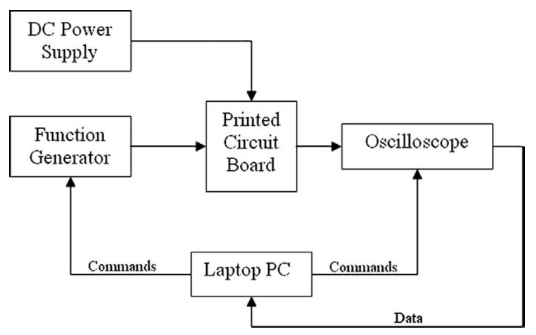
\includegraphics[width=6cm]
{Figure/oprindeligebd}}
\caption{Blokdiagram over det oprindelige kredsløb\cite{Aroom2009}}
\label{fig:oprindeligebd}
\end{figure}

\subsection{Strømforsyning}
I artiklen \cite{Aroom2009} blev der brugt en $\pm$12v strømforsyning tilsluttet til netforsyningen. Vi valgte at undgå netforsyningen, ved at sætte otte AA batterier i serie, både for +12v og -12v.

\begin{figure}[H]
\centering
{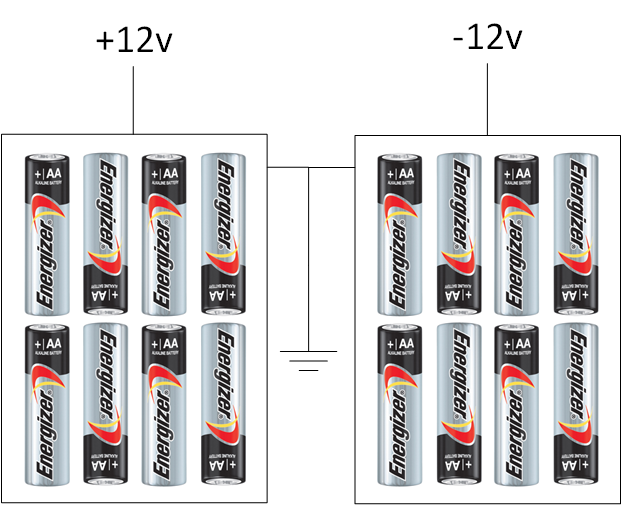
\includegraphics[width=10cm]
{Figure/12vbatteri}}
\caption{$\pm$12v batteriforsyning}
\label{fig:12vbatteri}
\end{figure}

\subsection{Funktionsgenerator}
Analog Discovery blev brugt som funktionsgenerator, da denne er nem og hurtig til at generere signaler. Den ønskede frekvens på 50 kHz blev brugt, da det er en brugt frekvens når der skal måles et synk\cite{Kusuhara2004}. Amplituden blev sat til 2V. 

\begin{figure}[H]
\centering
{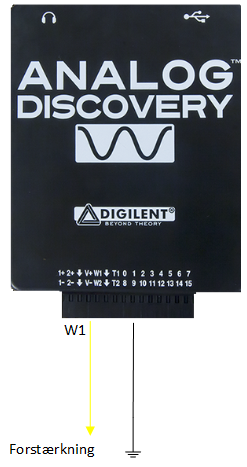
\includegraphics[width=6cm]
{Figure/analogdis}}
\caption{Analog discovery som funktionsgenerator}
\label{fig:analogdis}
\end{figure}


\subsection{Forstærkning}
Signalet fra Analog Discovery går ind til forstærkeren INA128. Den tilhørende gain modstand på 51kohm blev også brugt, da det giver en fordobling i forstærkning. På udgangen af INA128 er der nu 4V.

\begin{figure}[H]
\centering
{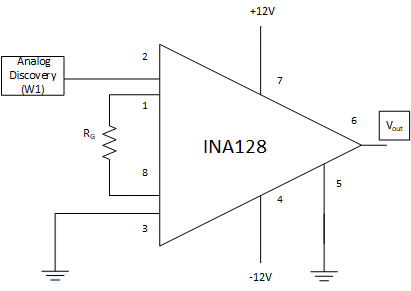
\includegraphics[width=10cm]
{Figure/ina128}}
\caption{Diagram over INA128}
\label{fig:ina128}
\end{figure}


\begin{figure}[H]
\centering
{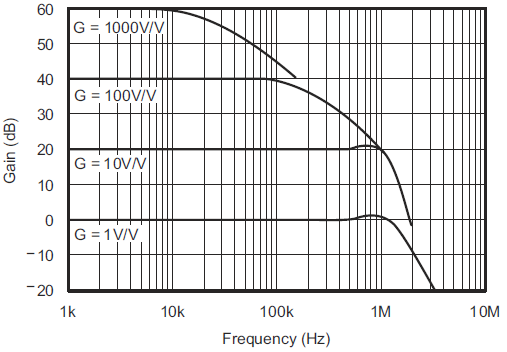
\includegraphics[width=10cm]
{Figure/ina128gain}}
\caption{Oversigt over hvilke frekvenser INA128 kan arbejde indenfor ved bestemte gains}
\label{fig:ina128gain}
\end{figure}

Ved en gain på 2 kan der aflæses i figur \ref{fig:ina128gain}, at båndbredden er over 100kHz, hvilket er indenfor den ønskede frekvens på 50kHz. 

\subsection{Strømgenerator}

\begin{figure}[H]
\centering
{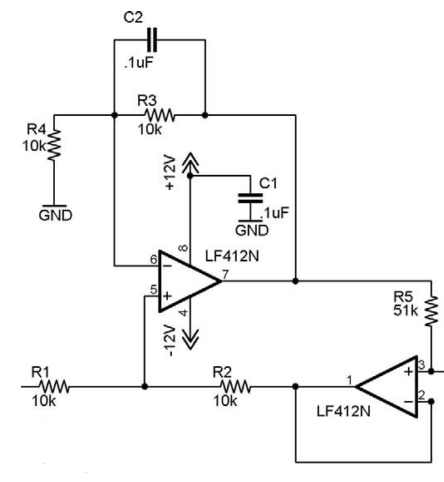
\includegraphics[width=10cm]
{Figure/howland1}}
\caption{Diagram over VCCS. Den faste spænding på 4V til VCCS giver en fast strøm på 100uA}
\label{fig:howland1}
\end{figure}

Spændningen kommer ind ved modstand R1 og strømmen ud på ben 3 på LF412N. Kombinationen af bestemt ohmsk modstand størrelse og lav \% tolerance modstand giver den faste strøm. Her er der brugt 1\% modstande. Ved at ændre modstand R5, kan en ønsket strøm beregnes\cite{Aroom2009}: $$I_{tissue}=2*\frac{V_{in}}{R_{5}}$$


\subsection{Elektroder}

\begin{figure}[H]
\centering
{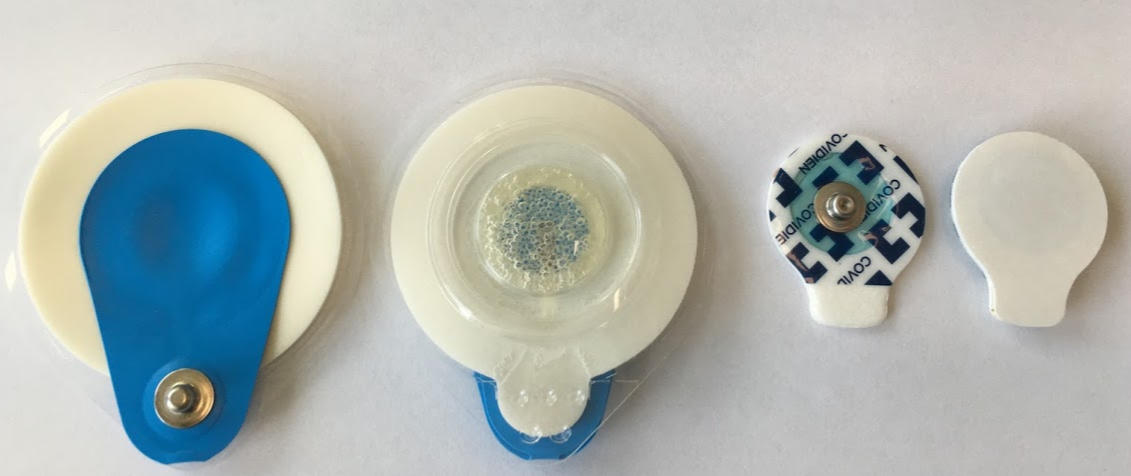
\includegraphics[width=12cm]
{Figure/elektroder}}
\caption{Ved målingerne er der blevet brugt EKG elektroder (venstre) og EMG elektroder (højre).}
\label{fig:elektroder}
\end{figure}

De forskellige elektroder kan ses i figur \ref{fig:elektroder}. EKG elektroderne er nemme at påsætte og indeholder meget gel som giver optimal kontakt, men fysisk fylder de meget. EMG elektroderne har mindre gel, men fylder næsten ingen ting. 






\subsection{A/D konverter}

Det analogt signal er blevet samplet ved brug af Analog Discovery som målte over elektroderne. Der blev også monteret et multimeter i serie for at aflæse den konstante strøm.


\begin{figure}[H]
\centering
{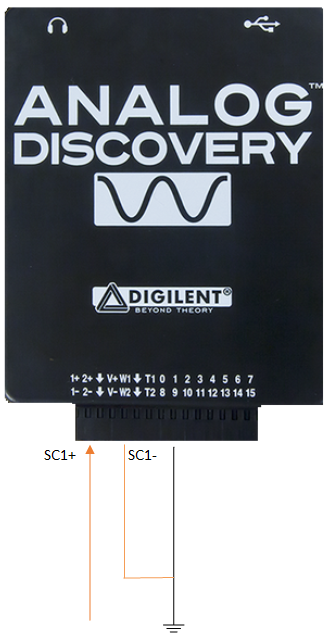
\includegraphics[width=6cm]
{Figure/adkonverter}}
\caption{Scope channel 1 positiv blev brugt til at måle spændingen over elektroderne}
\label{fig:adkonverter}
\end{figure}

\begin{figure}[H]
\centering
{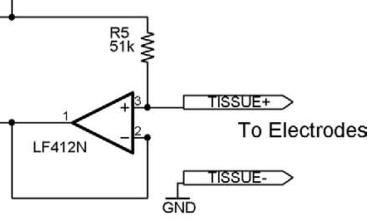
\includegraphics[width=6cm]
{Figure/elektroderdia}}
\caption{Der blev målt over elektroderne mellem ben 3 på LF412N og ground.}
\label{fig:elektroderdia}
\end{figure}

\section{Software}
\subsection{Waveforms}

\section{Testopstillinger}
\section{Konklusion}

\chapter{Det modificeret kredsløb}
\section{Hardware del 1 - Strømgenerator}
\subsection{Strømforsyning}
\subsection{Funktionsgenerator}
\subsection{Forstærkning}
\subsection{Strømgenerator}
\subsection{Elektroder}
\section{Hardware del 2 - Spændingsmåler}
\subsection{Strømforsyning}
\subsection{Elektroder}
\subsection{Forstærkning}
\subsection{Antialiaseringsfilter}
\subsection{A/D konverter}


\section{Software}
\subsection{Matlab}

\section{Testopstillinger}
\section{Konklusion}

\chapter{EMG}


\begin{figure}[H]
\centering
{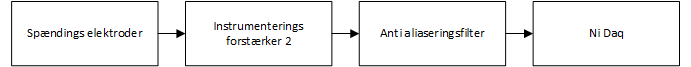
\includegraphics[width=\linewidth]
{Figure/analyse2}}
\caption{Bioimpedans ind}
\label{analyse2}
\end{figure}



\begin{figure}[H]
\centering
{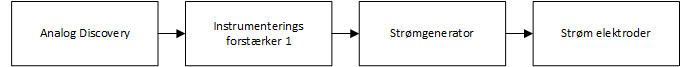
\includegraphics[width=\linewidth]
{Figure/analyse1}}
\caption{Bioimpedans ud}
\label{fig:analyse1}
\end{figure}

Instrumenterings forstærker 1\\
I det oprindelig design af BI konstateret vi at det var lavet lavet til at måle BI'er på skalpen og ikke over svælget. Derfor valgte vi at instrumenterings forstærkeren fik et større signal ind fra Analog Discovery på 2V og 50kHz. I det hele taget undrede vi over artiklens valg af brug af instrumenterings forstærker i starten af kredsløbet, da den ikke er et must for at realisere kredsløbet. Men dens eneste formål var at nedbringe common-mode støj fra funktions generatoren, så vi valgte at beholde denne da vi også vil undgå så meget støj som muligt videre i kredsløbet. Gain var oprindeligt sat til 51 Kohm hvilket giver det dobbelte af hvad instrumenterings forstærkeren tilføre. I diagrammet på figur \ref{BIdiagram} kan det ses at instrumenterings forstærkeren bliver forsynet med +12/-12 V, men der er her valgt at -12 V skal direkte til ground, hvilket har resulteret i at instrumenterings forstærkeren ikke fungerer korrekt, så der er den i stedet forsynet med -12 V og ikke ground.  





Strømgenerator\\
Det forstærket signal som kommer fra udgangen på instrumenterings forstærkeren løber over til strømgeneratoren. Denne strømgenerator er en Howland bridge. Sammensætningen af modstandene er vigtige og deres tolerance skal være lav for at få en korrekt og konstant strøm. For at justerer strømmen kan R5 udskiftes i kredsløbet. For at få en konstant strøm omkring ca. 500 uA, er modstanden ændret fra 51 Kohm til 2 Kohm.  

\textbf{Det oprindelige kredsløb}\\
Først bygges det oprindelige kredsløb som det er opgivet og der bliver foretaget en no load test, for at se om det stemmer overens med figuren fra artiklen.

\begin{figure}[H]
\centering
\begin{minipage}{.5\textwidth}
  \centering
  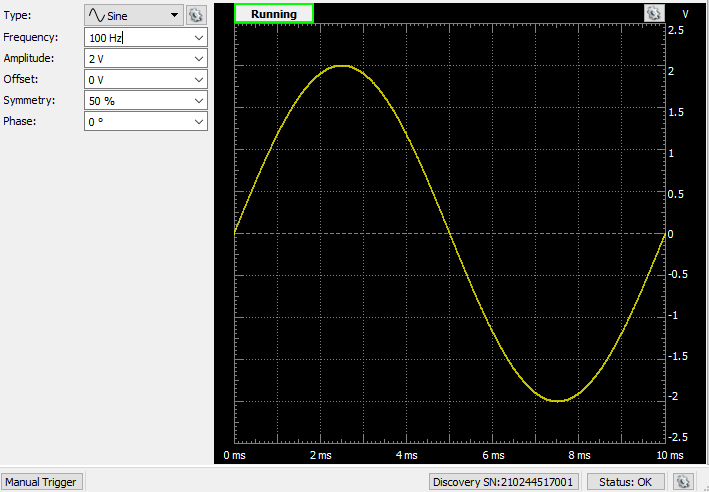
\includegraphics[width=.9\linewidth]{Figure/VCCSwavegen1}
  \captionof{figure}{A figure}
  \label{fig:test1}
\end{minipage}%
\begin{minipage}{.5\textwidth}
  \centering
  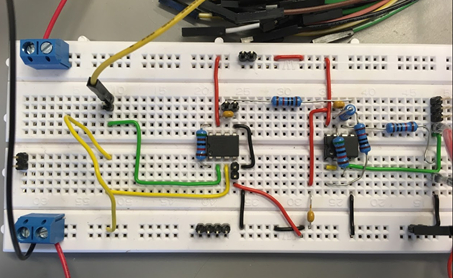
\includegraphics[width=.9\linewidth]{Figure/oprindeligekredslob}
  \captionof{figure}{Another figure}
  \label{fig:test2}
\end{minipage}
\end{figure}



\begin{table}[ht]
\begin{minipage}[b]{0.30\linewidth}
\centering
\begin{tabular}{ r |  r }
    \hline
    Hz & uA \\ \hline
    100 & 49 \\ \hline
    200 & 40 \\ \hline
    300 & 35 \\ \hline
    400 & 32 \\ \hline
    500 & 30 \\ \hline
    600 & 29 \\ \hline
    700 & 28 \\ \hline
    800 & 27 \\ \hline
    900 & 27 \\ \hline
    1000 & 27 \\ \hline
    2000 & 24 \\ \hline
    3000 & 21 \\ \hline
    4000 & 19 \\ \hline
    5000 & 17 \\ \hline
    6000 & 14 \\ \hline
    7000 & 12 \\ \hline
    8000 & 10 \\ \hline
    9000 & 7 \\ \hline
    10000 & 5 \\ \hline
    20000 & 0 \\ \hline
\end{tabular}
    \caption{Student Database}
    \label{table:student}
\end{minipage}\hfill
\begin{minipage}[b]{0.7\linewidth}
\centering
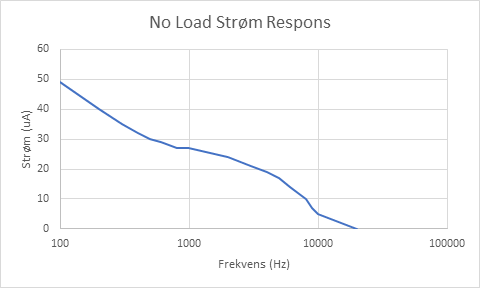
\includegraphics[width=10cm]{Figure/stromfrekvensoprindelig}
\captionof{figure}{2-D scatterplot of the Student Database}
\label{fig:image}
\end{minipage}
\end{table}


\textbf{Det modificeret kredsløb}\\

\begin{table}[H]
\begin{minipage}[b]{0.30\linewidth}
\centering
\begin{tabular}{ r |  r }
    \hline
    Hz & uA \\ \hline
    100 & 1268 \\ \hline
    200 & 1051 \\ \hline
    300 & 920 \\ \hline
    400 & 845 \\ \hline
    500 & 802 \\ \hline
    600 & 775 \\ \hline
    700 & 756 \\ \hline
    800 & 744 \\ \hline
    900 & 735 \\ \hline
    1000 & 728 \\ \hline
    2000 & 703 \\ \hline
    3000 & 696 \\ \hline
    4000 & 692 \\ \hline
    5000 & 688 \\ \hline
    6000 & 685 \\ \hline
    7000 & 683 \\ \hline
    8000 & 680 \\ \hline
    9000 & 678 \\ \hline
    10000 & 676 \\ \hline
    20000 & 675 \\ \hline
    30000 & 634 \\ \hline
    40000 & 596 \\ \hline
    50000 & 542 \\ \hline
    60000 & 475 \\ \hline
    70000 & 405 \\ \hline
    80000 & 332 \\ \hline
    90000 & 268 \\ \hline
    100000 & 210 \\ \hline
    110000 & 161 \\ \hline
    120000 & 120 \\ \hline
    130000 & 87 \\ \hline
    140000 & 60 \\ \hline
    150000 & 40 \\ \hline
    160000 & 25 \\ \hline
    170000 & 16 \\ \hline
    180000 & 10 \\ \hline
    190000 & 6 \\ \hline
    200000 & 4 \\ \hline
    210000 & 2 \\ \hline
    220000 & 1 \\ \hline
    230000 & 1 \\ \hline
    240000 & 0 \\ \hline
        
\end{tabular}
    \caption{Student Database}
    \label{table:student}
\end{minipage}\hfill
\begin{minipage}[b]{0.7\linewidth}
\centering
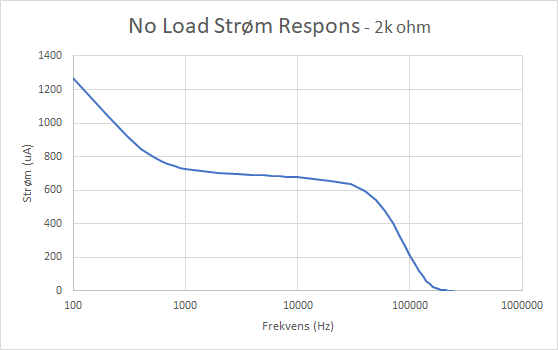
\includegraphics[width=10cm]{Figure/stromfrekvensoprindelig2k}
\captionof{figure}{2-D scatterplot of the Student Database}
\label{fig:image}
\end{minipage}
\end{table}














Overvejelser om mulige løsninger
løsninger I har valgt, begrundelsen herfor
grundlæggende valg af hardware- og softwaremæssige komponenter, som er kritiske for realisering af systemet

For at træffe et valg kan der analyseres og diskuteres forskellige løsninger mht. til ydeev-ne, pris, leveringstid og forhåndskendskab. Disse kan med fordel opstilles i tabelform.

Anti-alisering
Elektroder
Konstant strøm
Lavpas filtering
Ensretter
Sampling af signal \cite{martin}





\chapter{Konklusion}
\bibliography{library}

\end{document}
